\documentclass[a4paper,12pt]{article}

\usepackage[utf8]{inputenc}
\usepackage[T1]{fontenc}
\usepackage[portuguese]{babel}
\usepackage{amsmath}
\usepackage{booktabs}
\usepackage{graphicx}
\usepackage{geometry}
\geometry{margin=2.5cm}
\usepackage{xcolor}
\usepackage{listings}
\usepackage{hyperref}
\usepackage{float}
\usepackage{tabularx}
\usepackage{array}
\hypersetup{colorlinks=true, linkcolor=blue!50!black, urlcolor=blue!50!black}
\renewcommand{\tablename}{Tabela}
\renewcommand{\lstlistingname}{Código}
\newcolumntype{Y}{>{\raggedright\arraybackslash}X}

% ---------- Configuração do realce de sintaxe (C) ----------
\definecolor{codebg}{RGB}{247,247,247}
\definecolor{codekw}{RGB}{0,0,180}
\definecolor{codecomment}{RGB}{0,128,0}
\definecolor{codestring}{RGB}{163,21,21}
\definecolor{framecolor}{RGB}{200,200,200}

\lstdefinestyle{cstyle}{
    language=C,
    backgroundcolor=\color{codebg},
    basicstyle=\ttfamily\footnotesize,
    keywordstyle=\color{codekw}\bfseries,
    commentstyle=\color{codecomment}\itshape,
    stringstyle=\color{codestring},
    numberstyle=\tiny\color{gray},
    numbers=left,
    numbersep=6pt,
    frame=single,
    rulecolor=\color{framecolor},
    breaklines=true,
    breakatwhitespace=false,
    showstringspaces=false,
    tabsize=4,
    captionpos=b,
    columns=flexible,
    morekeywords={size_t},
    extendedchars=true,
    literate=
        {á}{{\'a}}1 {à}{{\`a}}1 {â}{{\^a}}1 {ã}{{\~a}}1
        {é}{{\'e}}1 {ê}{{\^e}}1 {í}{{\'i}}1
        {ó}{{\'o}}1 {ô}{{\^o}}1 {õ}{{\~o}}1
        {ú}{{\'u}}1 {ü}{{\"u}}1 {ç}{{\c c}}1
        {Á}{{\'A}}1 {À}{{\`A}}1 {Â}{{\^A}}1 {Ã}{{\~A}}1
        {É}{{\'E}}1 {Ê}{{\^E}}1 {Í}{{\'I}}1
        {Ó}{{\'O}}1 {Ô}{{\^O}}1 {Õ}{{\~O}}1
        {Ú}{{\'U}}1 {Ü}{{\"U}}1 {Ç}{{\c C}}1
}

\title{Tarefa 14: Programação em Memória Distribuída}
\author{Israel Soares de Castro Filho \\ Matrícula: 20250070780}
\date{}

\begin{document}

\maketitle

\section{Introdução}

Em programação paralela com memória distribuída, o custo de comunicar uma mensagem
entre dois processos depende de duas características do sistema: a
\emph{latência} ($\alpha$), tempo fixo para iniciar qualquer comunicação, e a
\emph{largura de banda} ($\beta$), taxa sustentada de transferência de dados.
Um modelo simples e muito usado para o tempo de uma mensagem unidirecional de $n$
bytes é o modelo de Hockney:
\begin{equation}
    T(n) = \alpha + \frac{n}{\beta}.
\end{equation}
Este trabalho mede $T(n)$ com um teste de \emph{ping-pong} em MPI, executado no
supercomputador NPAD (UFRN), e identifica os regimes em que a latência domina
(mensagens pequenas) e em que a largura de banda domina (mensagens grandes).

\section{Metodologia}

O programa (Código~\ref{lst:tarefa14}, no Apêndice) usa exatamente dois processos.
O processo 0 envia uma mensagem de $n$ bytes ao processo 1 com \texttt{MPI\_Send}, e
o processo 1 a devolve imediatamente com \texttt{MPI\_Send}, enquanto o processo 0
a recebe com \texttt{MPI\_Recv}. O tempo de várias trocas consecutivas é medido com
\texttt{MPI\_Wtime}, após um \texttt{MPI\_Barrier}.

Detalhes do experimento:
\begin{itemize}
    \item tamanhos de $8$ bytes ($\approx 10^1$) a $64$ MiB ($\approx 7\times 10^7$ bytes), em potências de 2 ($2^3$ a $2^{26}$);
    \item número de repetições adaptativo por tamanho (de $20$ a $20\,000$ idas e
          voltas), para que cada medição tenha duração suficiente;
    \item $20$ trocas de aquecimento não medidas e $5$ tentativas por tamanho,
          sendo registrada a de menor tempo (para reduzir ruído);
    \item o buffer é inicializado antes da medição (evita \emph{page faults}) e o
          conteúdo devolvido é verificado ao final de cada tentativa;
    \item o tempo unidirecional é $T(n)=t_{\text{total}}/(2\cdot\text{reps})$ e a
          banda efetiva é $n/T(n)$.
\end{itemize}

O experimento foi executado em dois cenários no NPAD, com o script bash (\ref{lst:bash}):

\begin{enumerate}
    \item \textbf{intra-nó}, com os dois processos no mesmo
    nó (comunicação via memória compartilhada)
    \item \textbf{inter-nó}, com um
    processo em cada nó (comunicação pela rede de interconexão).
    
\end{enumerate}

Os resultados foram
processados com \texttt{plot\_pingpong.py}, que também ajusta o modelo de Hockney por
mínimos quadrados com pesos $1/T$ (erro relativo) e calcula
$n_{1/2}=\alpha\beta$, o tamanho a partir do qual o termo de banda supera o de
latência.

\section{Resultados}

\begin{figure}[H]
    \centering
    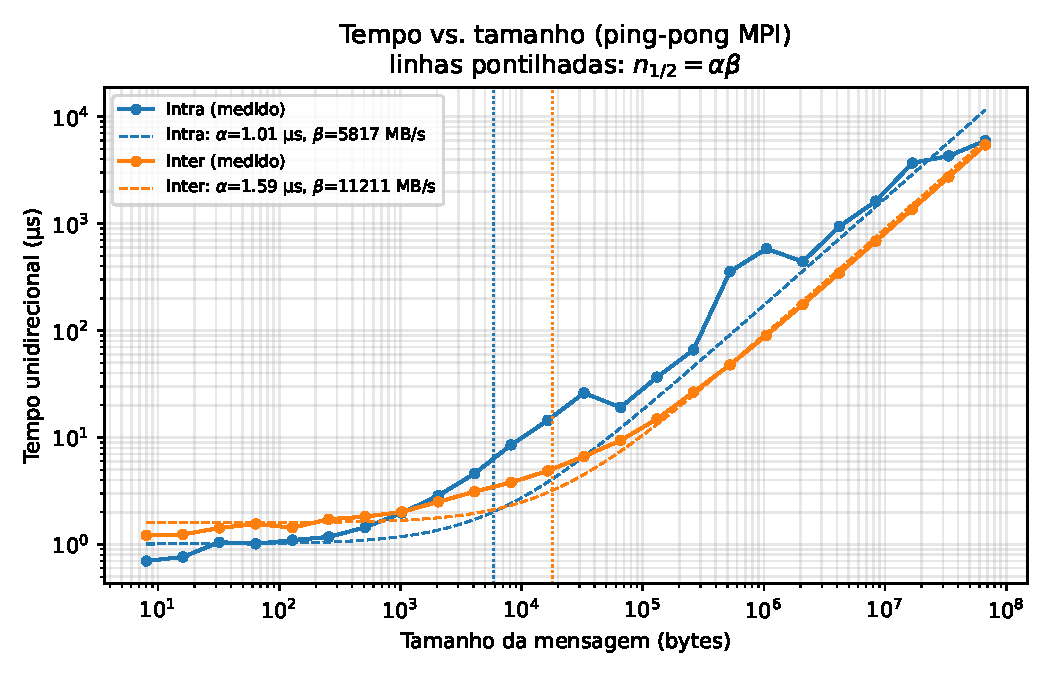
\includegraphics[width=0.8\textwidth]{../graficos/grafico_tempo.pdf}
    \caption{Tempo unidirecional em função do tamanho da mensagem (escala
    log-log), com ajuste do modelo de Hockney.}
    \label{fig:tempo}
\end{figure}

\begin{figure}[H]
    \centering
    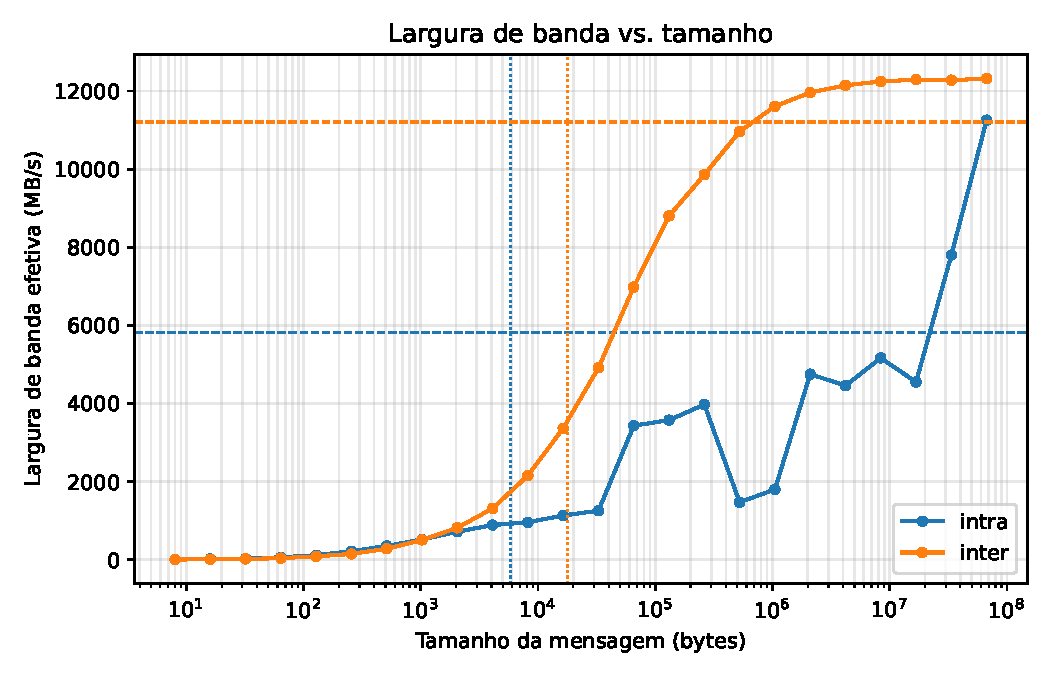
\includegraphics[width=0.8\textwidth]{../graficos/grafico_banda.pdf}
    \caption{Largura de banda efetiva em função do tamanho da mensagem.}
    \label{fig:banda}
\end{figure}

\begin{table}[H]
    \centering
    \begin{tabular}{lrrr}
        \toprule
        Cenário & $\alpha$ ($\mu$s) & $\beta$ (MB/s) & $n_{1/2}$ (bytes) \\
        \midrule
        Intra-nó & 1.008 & 5816.5 & 5865 \\
        Inter-nó & 1.591 & 11210.8 & 17835 \\
        \bottomrule
    \end{tabular}
    \caption{Parâmetros do modelo de Hockney ajustados.}
    \label{tab:hockney}
\end{table}

\section{Análise}

\subsection{Como ler os gráficos}

No eixo horizontal, cada marca é $10$ vezes maior que a anterior
($10^1, 10^2, \dots, 10^8$ bytes). No gráfico de tempo, quanto mais alta a
curva, mais lenta a comunicação; no de banda, quanto mais alta, melhor.
Os valores abaixo são aproximados, lidos dos gráficos (exceto os da
Tabela~\ref{tab:hockney}).

\subsection{Os dois regimes (inter-nó)}

\begin{table}[H]
    \centering
    \begin{tabularx}{\textwidth}{@{}l l Y@{}}
    \toprule
        Regime & Tamanho da mensagem & O que se vê \\
    \midrule
        Latência domina & até $\approx 10^3$ bytes &
            o tempo quase não muda ($\approx 1{,}2$ a $2~\mu$s); a banda é
            menor que $5\%$ do pico \\
        Transição & $\approx 10^3$ a $\approx 10^5$ bytes &
            latência e banda pesam parecido \\
        Banda domina & a partir de $\approx 10^5$ bytes &
            o tempo cresce na mesma proporção do tamanho; a banda sobe até
            $\approx 12{,}3$~GB/s ($>90\%$ do pico em $\approx 10^6$ bytes) \\
    \bottomrule
    \end{tabularx}
    \caption{Resumo dos regimes no cenário inter-nó.}
    \label{tab:regimes}
\end{table}

Simplificando:
\begin{itemize}
    \item \textbf{Mensagens pequenas} (até $\approx 10^3$ bytes): mandar $10$
          bytes ou $1000$ bytes leva quase o mesmo tempo. O que pesa é o
          custo fixo de iniciar a comunicação, a \textbf{latência}.
    \item \textbf{Mensagens grandes} ($\approx 10^5$ bytes ou mais): o tempo
          passa a ser proporcional ao tamanho. O que pesa é transmitir os
          dados, a \textbf{largura de banda}. Em $\approx 7\times 10^7$ bytes,
          a latência é menos de $0{,}1\%$ do tempo.
    \item \textbf{Ponto de equilíbrio:}
          $n_{1/2}=\alpha\beta\approx 1{,}8\times 10^4$ bytes
          (Tabela~\ref{tab:hockney}), no meio da faixa de transição.
\end{itemize}

\begin{table}[H]
    \centering
    \begin{tabular}{rrrrr}
    \toprule
        & \multicolumn{2}{c}{Inter-nó} & \multicolumn{2}{c}{Intra-nó} \\
        \cmidrule(lr){2-3} \cmidrule(lr){4-5}
        Tamanho (bytes) & Tempo ($\mu$s) & Banda (MB/s) & Tempo ($\mu$s) & Banda (MB/s) \\
    \midrule
        $8$ ($\approx 10^1$)               & $\approx 1{,}2$ & $\approx 7$      & $\approx 0{,}7$ & $\approx 11$ \\
        $1\,024$ ($\approx 10^3$)          & $\approx 2$     & $\approx 500$    & $\approx 2$     & $\approx 500$ \\
        $131\,072$ ($\approx 10^5$)        & $\approx 15$    & $\approx 8\,800$ & $\approx 35$    & $\approx 3\,600$ \\
        $1\,048\,576$ ($\approx 10^6$)     & $\approx 90$    & $\approx 11\,600$& $\approx 580$   & $\approx 1\,800$ \\
        $8\,388\,608$ ($\approx 10^7$)     & $\approx 700$   & $\approx 12\,200$& $\approx 1\,600$& $\approx 5\,200$ \\
    \bottomrule
    \end{tabular}
    \caption{Pontos de referência (tempo unidirecional e banda efetiva),
    aproximados e lidos dos gráficos.}
    \label{tab:pontos}
\end{table}

\subsection{Intra-nó vs. inter-nó}

\begin{itemize}
    \item \textbf{Mensagens pequenas} ($\approx 10^1$ bytes): o intra-nó é mais
          rápido ($\approx 0{,}7~\mu$s contra $\approx 1{,}2~\mu$s), pois não
          passa pela rede.
    \item \textbf{A partir de $\approx 10^5$ bytes:} o inter-nó é melhor. O
          intra-nó dá um salto entre $10^5$ e $10^6$ bytes
          ($\approx 5\times 10^5$), onde o inter-nó é cerca de $7$ vezes mais
          rápido.
    \item \textbf{Modelo de Hockney:} descreve bem o inter-nó e mal o
          intra-nó, que é irregular; $\beta$ e $n_{1/2}$ do intra-nó são só
          aproximados.
    \item \textbf{Causas possíveis} (hipóteses): cópia extra
          pela memória, efeitos de cache e posicionamento dos processos nos
          soquetes.
\end{itemize}

\section{Conclusão}

\begin{itemize}
    \item A \textbf{latência domina} até $\approx 10^3$ bytes e a
          \textbf{largura de banda domina} a partir de $\approx 10^5$ bytes.
          O equilíbrio fica em $n_{1/2}\approx 1{,}8\times 10^4$ bytes
          (inter-nó).
    \item Números principais (inter-nó): $\alpha\approx 1{,}6~\mu$s e
          $\beta\approx 11{,}2$~GB/s (patamar medido de $\approx 12{,}3$~GB/s).
    \item \textbf{Na prática:} Enviar $1024$
          mensagens de $8$ bytes custa $\approx 1{,}2$~ms, contra
          $\approx 3{,}7~\mu$s para uma única mensagem com os mesmos
          $\approx 8\times 10^3$ bytes (mais de $300$ vezes menos).
    \item O intra-nó tem latência menor, mas desempenho irregular para
          mensagens médias e grandes.
\end{itemize}

\newpage
\appendix

\section{Código-Fonte}

\lstinputlisting[style=cstyle, caption={Ping-pong MPI (\texttt{tarefa14.c}).}, label={lst:tarefa14}]{../src/tarefa14.c}

\lstinputlisting[style=cstyle, caption={Script bash (\texttt{tarefa14.sh})}, label={lst:bash}]{../src/tarefa14.sh}

\end{document}